
\chapter{Estudo de simulação}\label{cap:simulacao}

%=====================================================

Com o objetivo de avaliar o poder do teste Wald em testes de hipóteses sobre parâmetros de McGLMs, foram executados estudos de simulação. Nestas simulações avaliamos o comportamento da proposta para três distribuições de probabilidade: Normal, Poisson e Bernoulli. Simulamos cenários univariados e também trivariados com diferentes tamanhos amostrais para verificar as propriedades dos testes sobre parâmetros de regressão e dispersão.

Para simular conjuntos de dados univariados foram usadas bibliotecas padrões do R. Para simular conjuntos de dados com múltiplas respostas seguindo distribuição Normal, foi usada a biblioteca R \emph{mvtnorm} \citep{mvtnorm1}, \citep{mvtnorm2}. Para as outras distribuições foi utilizado o método NORTA \citep{cario1997modeling} implementado na biblioteca R \emph{NORTARA} \citep{nortara}.

\section{Parâmetros de regressão}

Para avaliação de hipóteses sobre parâmetros de regressão foram considerados tamanhos amostrais de 50, 100, 250, 500 e 1000. Foram gerados 500 conjuntos de dados para cada tamanho amostral simulando uma situação com uma variável explicativa categórica de 4 níveis. Para distribuição Normal os parâmetros de regressão usados foram: $\beta_0 = 5$, $\beta_1 = 0$, $\beta_2 = 0$, $\beta_3 = 0$. Para a distribuição Poisson os parâmetros de regressão usados foram: $\beta_0 = 2,3$, $\beta_1 = 0$, $\beta_2 = 0$, $\beta_3 = 0$. E para a distribuição Bernoulli os parâmetros de regressão usados foram: $\beta_0 = 0,5$, $\beta_1 = 0$, $\beta_2 = 0$, $\beta_3 = 0$. Os valores foram escolhidos de tal modo que o coeficiente de variação para distribuição Normal fosse de 20\%, as contagens para Poisson fossem próximas de 10 e a probabilidade de sucesso da Bernoulli fosse aproximadamente 0,6. Foram avaliados cenários univariados e trivariados com estas características. Para os cenários trivariados, existem 4 parâmetros por resposta que seguem as configurações descritas. Para cada amostra gerada foi ajustado um McGLM nos quais as funções de ligação e variância para cada distribuição são apresentadas na \autoref{tab:link_var}. 

\begin{table}[H]
\centering
\begin{tabular}{ccc}
\hline
Distribuição & Função de ligação & Função de variância \\ \hline
Normal       & Identidade        & Constante           \\
Poisson      & Logarítmica       & Tweedie             \\
Bernoulli    & Logito            & Binomial            \\ \hline
\end{tabular}
\caption{Funções de ligação e variância utilizadas nos modelos para cada distribuição simulada.}
\label{tab:link_var}
\end{table}

Em todos os casos o preditor matricial para a matriz de variância e covariância foi especificado de forma a explicitar que as observações são independentes dentro de cada resposta. A correlação entre respostas no caso trivariado é dada pela matriz $\Sigma_b$ descrita na \autoref{eq:correlacao}.

\begin{equation} \label{eq:correlacao}
\Sigma_b = 
\begin{bmatrix}
1    & 0,75 & 0,5  \\
0,75 & 1    & 0,25 \\
0,5  & 0,25 & 1    \\
\end{bmatrix}
\end{equation}

Com os modelos ajustados, o procedimento consistiu em variar as hipóteses testadas sobre os parâmetros simulados. Consideramos 20 diferentes hipóteses baseadas em um decréscimo em $\beta_0$ e distribuição deste decréscimo nos demais $\beta$s da hipótese nula. O decréscimo para respostas seguindo distribuição Normal foi de 0,15; para distribuição Poisson o decréscimo foi de 0,05; e para distribuição Bernoulli o decréscimo foi de 0,25. Estes valores foram escolhidos levando em conta o o afastamento desejado das hipóteses testadas na escala da resposta e é importante notar que estes valores são diferentes devido ao impacto da função de ligação usada em cada configuração de modelo e também devido às propriedades dos parâmetros das distribuições.

Para cada ponto avaliamos o percentual de rejeição da hipótese nula. A ideia é verificar o que ocorre quando afastamos as hipóteses nulas dos reais valores dos parâmetros. Espera-se que no primeiro ponto haja um percentual de rejeição baixo, pois a hipótese nula corresponde aos reais valores dos parâmetros. Para os demais pontos espera-se que o percentual de rejeição aumente gradativamente, pois as hipóteses afastam-se cada vez mais dos valores originalmente simulados. As hipóteses testadas em cada cenário estão disponíveis no apêndice desta dissertação.
 
Para representar graficamente os resultados tomamos a distância euclideana de cada vetor de hipóteses com relação ao vetor usado para simular os dados. Adicionalmente dividimos o vetor de distâncias pela maior distância para obter distâncias padronizadas entre 0 e 1, independente dos parâmetros de regressão. Os resultados são apresentados na \autoref{fig:betas}.

\begin{figure}[H]
\centering
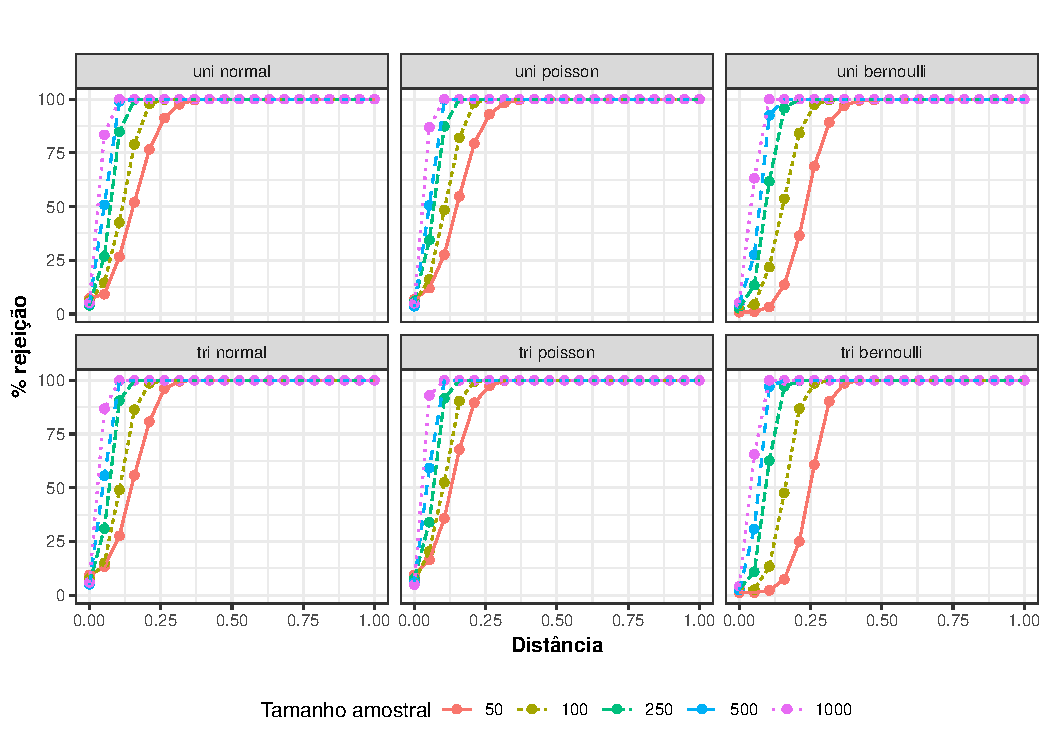
\includegraphics[width=15cm]{/home/lacf14/msc/4_dissertacao/6-simulacao/betas.pdf}
\caption{Resultados do estudo de simulação para os parâmetros de regressão.}
\label{fig:betas}
\end{figure}

De modo geral, quanto mais distante a hipótese é dos valores inicialmente simulados, maior é o percentual de rejeição. Como esperado, os menores percentuais foram observados na hipótese igual aos valores simulados. Nos cenários univariados o percentual de rejeição foi próximo de 5\% quando a hipótese era igual aos valores simulados mesmo com tamanhos amostrais reduzidos. Para os cenários trivariados, no menor tamanho amostral avaliado, o percentual de rejeição não excedeu 10\% e em tamanhos amostrais iguais a 500 o percentual de rejeição foi próximo de 5\%. Também como esperado, foi possível verificar que conforme aumenta-se o tamanho amostral, o percentual de rejeição aumenta para hipóteses pouco diferentes dos valores simulados dos parâmetros.

\section{Parâmetros de dispersão}

Para avaliação de hipóteses sobre parâmetros de dispersão foram considerados os mesmos tamanhos amostrais: 50, 100, 250, 500 e 1000. Contudo, os conjuntos de dados simulam uma situação em que cada unidade amostral fornece 5 medidas ao conjunto de dados. Foram gerados 500 conjuntos de dados para cada tamanho amostral e distribuição. Para distribuição Normal foram simulados vetores com média 5 e desvio padrão igual a 1. Para distribuição Poisson foram simuladas contagens com taxa igual a 10. Para distribuição Bernoulli foram simulados vetores de uma variável dicotômica com probabilidade de sucesso igual a 0,6.

Em todos os casos, os parâmetros de dispersão para gerar os conjuntos de dados foram fixados em $\tau_0 = 1$, $\tau_1 = 0$ e não foi incluído efeito de variáveis explicativas. Foram avaliados cenários univariados e trivariados com estas características. Para cada amostra gerada foi ajustado um McGLM com funções de ligação e variância tal como descrito na \autoref{tab:link_var}. Nos cenários trivariados a correlação entre respostas é dada pela \autoref{eq:correlacao}.

Neste caso, como o objetivo é avaliar a correlação dentro das respostas, é necessário especificar um preditor matricial. O objetivo é testar hipóteses sobre os parâmetros de dispersão associados a este preditor matricial. 

Com os modelos ajustados, o procedimento consistiu em variar as hipóteses testadas sobre os parâmetros simulados. Consideramos 20 diferentes hipóteses baseadas em um decréscimo sucessivo de 0,02 em $\tau_0$ e acréscimo de 0,02 em $\tau_1$ para cada hipótese nula testada. Para cada ponto avaliamos o percentual de rejeição da hipótese nula. A ideia é afastar sucessivamente a hipótese dos valores simulados e avaliar se conforme afastamos a hipótese dos valores verdadeiros, o percentual de rejeição aumenta. As hipóteses testadas estão disponíveis no apêncice.

Do mesmo modo que foi feito para os parâmetros de regressão, foi tomada a distância euclideana de cada vetor de hipóteses com relação ao vetor usado para simular os dados; e o vetor de distâncias foi padronizado para obter distâncias entre 0 e 1. Os resultados são apresentados na \autoref{fig:taus}.

\begin{figure}[H]
\centering
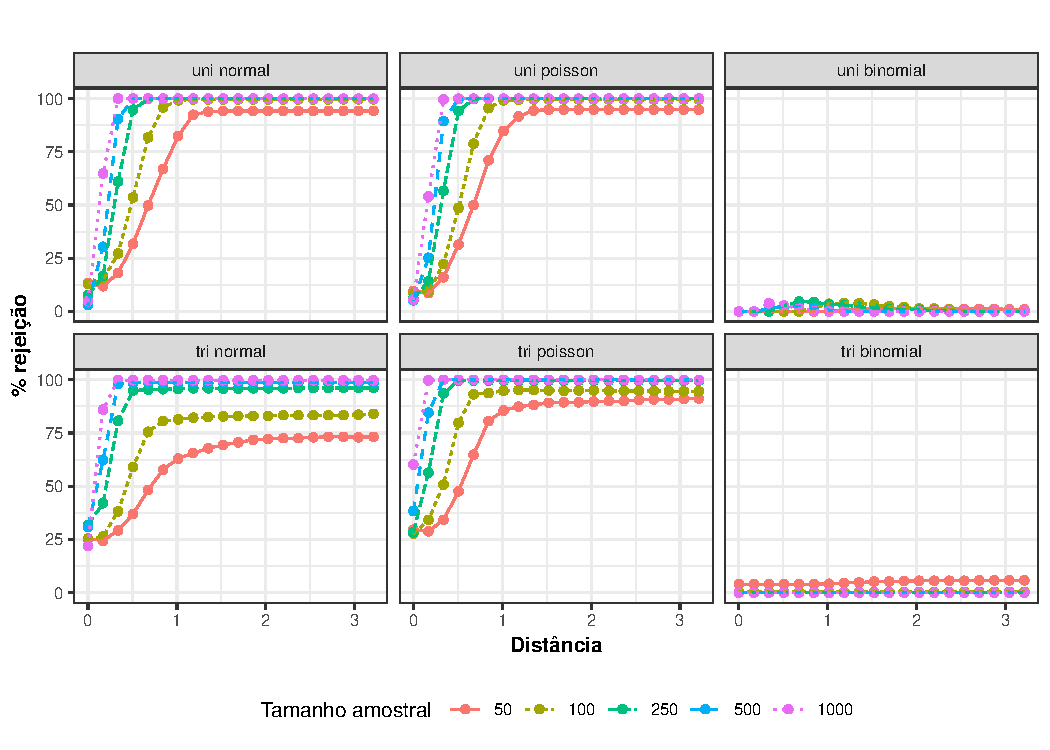
\includegraphics[width=15cm]{/home/lacf14/msc/4_dissertacao/6-simulacao/taus.pdf}
\caption{Resultados do estudo de simulação para os parâmetros de dispersão.}
\label{fig:taus}
\end{figure}

Assim como observado para os parâmetros de regressão, o comportamento dos gráficos mostra que, quanto mais distante a hipótese é dos valores inicialmente simulados, maior é o percentual de rejeição, e os menores percentuais são observados em hipóteses próximas aos valores simulados. Na primeira hipótese testada, para os cenários univariados, percentuais de rejeição próximos a 8\% na primeira hipótese foram observados no menor tamanho amostral avaliado. A partir de tamanhos amostrais iguais a 250 o percentual de rejeição foi próximo de 5\%. Já para os casos trivariados, no menor tamanho amostral, o percentual de rejeição excedia 10\% no menor tamanho amostral; para tamanhos amostrais maiores, os percentuais ficaram em torno de 7\%. Também verificou-se para parâmetros de dispersão que conforme aumenta-se o tamanho amostral, o percentual de rejeição aumenta para hipóteses pouco diferentes dos valores simulados dos parâmetros.

%=====================================================